\chapter{Gruppengeschwindigkeit, fermionisches Ausschlussprinzip und Dirac-See}

\section{Phasengeschwindigkeit und Gruppengeschwindigkeit}

\begin{classroomqa}
\lecturetimestamp{00:00:07}
\audiencequestion{Was sind Gruppen- und Phasengeschwindigkeit?}
\lecturerresponse{Die Phasengeschwindigkeit beschreibt die Bewegung eines Punktes fester Phase in einer ebenen Welle. Im Allgemeinen beschreibt sie nicht die Bewegung eines messbaren Objekts. Die Gruppengeschwindigkeit beschreibt die Bewegung der Einhüllenden eines Wellenpakets und ist die Geschwindigkeit, die Teilchen, Signalen und dem Wahrscheinlichkeitsstrom zugeordnet ist.}
\end{classroomqa}

Man beginne mit einer ebenen Welle,
\begin{equation}
\psi(x,t)=e^{i(kx-\omega t)},
\end{equation}
oder mit ihrer reellen Form,
\begin{equation}
\psi(x,t)=\sin(kx-\omega t).
\end{equation}
Ein Wellenberg, ein Wellental oder ein anderer Punkt fester Phase bewegt sich so, dass
\begin{equation}
kx-\omega t=\text{constant}.
\end{equation}
Wählt man der Einfachheit halber die Konstante gleich null, erhält man
\begin{equation}
x=\frac{\omega}{k}t,
\qquad
v_{\mathrm{phase}}=\frac{\omega}{k}.
\end{equation}
Da \(\omega=2\pi/T\) und \(k=2\pi/\lambda\) gilt,
\begin{equation}
v_{\mathrm{phase}}=\frac{\omega}{k}=\frac{\lambda}{T}.
\end{equation}
Dies ist gerade die Strecke, um die eine bestimmte Phase während einer Periode voranschreitet.

Für eine nichtrelativistische Schr\"odinger-Welle mit \(\hbar=1\) sind Energie und Impuls \(\omega\) und \(k\), also gilt
\begin{equation}
\omega(k)=\frac{k^2}{2m}.
\end{equation}
Ihre Phasengeschwindigkeit ist daher
\begin{equation}
v_{\mathrm{phase}}=\frac{k}{2m}.
\end{equation}
Die gewöhnliche Geschwindigkeit eines Teilchens mit Impuls \(k\) ist dagegen \(k/m\). Die Abweichung um den Faktor zwei ist der erste Hinweis darauf, dass die Bewegung einer ebenen Wellenphase nicht der Bewegung des Teilchens entspricht.

Es gibt einen noch deutlicheren Hinweis. Man addiere dieselbe Konstante \(C\) zu jeder Frequenz:
\begin{equation}
\omega(k)\longrightarrow \omega(k)+C.
\end{equation}
Die Konstante könnte beispielsweise einen gemeinsamen Beitrag zur Ruheenergie wie \(mc_{\mathrm{light}}^2\) darstellen; ihre konkrete Bezeichnung ist jedoch unwichtig. Hier ist \(C\) eine Energieverschiebung und nicht die Lichtgeschwindigkeit. Die Phasengeschwindigkeit ändert sich dadurch zu
\begin{equation}
v_{\mathrm{phase}}\longrightarrow
\frac{\omega(k)+C}{k}
=v_{\mathrm{phase}}+\frac{C}{k}.
\end{equation}
Doch wenn man dieselbe Konstante zu jeder Energie addiert, ändern sich keine Energiedifferenzen und damit auch keine nichtrelativistische Physik.

Das lässt sich unmittelbar an der Wellenfunktion erkennen. Man schreibt ein allgemeines Schr\"odinger-Feld als Summe oder Integral über Moden,
\begin{equation}
\psi(x,t)=\sum_k a_k e^{ikx}e^{-i\omega(k)t},
\end{equation}
wobei Normierungsfaktoren weggelassen sind. Nach der Verschiebung gilt
\begin{align}
\psi(x,t)
&\longrightarrow
\sum_k a_k e^{ikx}e^{-i[\omega(k)+C]t}
\\
&=e^{-iCt}\psi(x,t).
\end{align}
Jede Mode hat dieselbe zeitabhängige Phase erhalten. Das konjugierte Feld erhält die entgegengesetzte Phase, sodass
\begin{equation}
\begin{aligned}
\psi^*(x,t)\psi(x,t)
&\longrightarrow
e^{iCt}e^{-iCt}\psi^*(x,t)\psi(x,t)
\\
&=\psi^*(x,t)\psi(x,t).
\end{aligned}
\end{equation}
Dieselbe Auslöschung tritt bei Erwartungswerten auf. Eine Größe, die sich bei einer Verschiebung des Energienullpunkts ändert, kann nicht die physikalische Ausbreitungsgeschwindigkeit des Schr\"odinger-Teilchens sein. Die Phasengeschwindigkeit ist daher teilweise konventionsabhängig.

Ein lokalisiertes Teilchen wird nicht durch eine einzelne unendlich ausgedehnte ebene Welle, sondern durch ein Wellenpaket dargestellt. Die Komponentenwellen überlagern sich im Bereich des Pakets konstruktiv und außerhalb davon destruktiv. Die Bewegung dieses Musters lässt sich bereits anhand zweier benachbarter Wellen bestimmen:
\begin{equation}
\psi(x,t)=
\sin(kx-\omega t)+
\sin(k'x-\omega't),
\end{equation}
wobei \(k'\) nahe bei \(k\) liegt und \(\omega'=\omega(k')\) gilt. Konstruktive Interferenz tritt dort auf, wo ihre Phasen übereinstimmen:
\begin{equation}
kx-\omega t=k'x-\omega't.
\end{equation}
Daraus folgt
\begin{equation}
(k-k')x=(\omega-\omega')t,
\end{equation}
und das sich verstärkende Muster bewegt sich gemäß
\begin{equation}
x=\frac{\omega-\omega'}{k-k'}t.
\end{equation}
Im Grenzfall benachbarter Wellen erhält man
\begin{equation}
x=\frac{d\omega}{dk}t,
\qquad
v_{\mathrm{group}}=\frac{d\omega}{dk}.
\end{equation}
Dies ist die Geschwindigkeit der Einhüllenden---des lokalisierten Wellenpakets, das durch die Interferenz der Komponentenwellen entsteht.

Für die nichtrelativistische Dispersionsrelation einschließlich der beliebigen Verschiebung
\begin{equation}
\omega(k)=\frac{k^2}{2m}+C,
\end{equation}
ist die Gruppengeschwindigkeit
\begin{equation}
v_{\mathrm{group}}
=\frac{d}{dk}\left(\frac{k^2}{2m}+C\right)
=\frac{2k}{2m}
=\frac{k}{m}.
\end{equation}
Die additive Konstante ist verschwunden, und das Ergebnis ist genau die klassische Teilchengeschwindigkeit.

\begin{classroomqa}
\lecturetimestamp{00:16:35}
\audiencequestion{Verschwindet der Faktor zwei bei der Gruppengeschwindigkeit?}
\lecturerresponse{Ja. Die Ableitung von \(k^2\) ergibt \(2k\); dadurch kürzt sich der Faktor zwei in \(2m\) heraus. Das Ergebnis ist \(k/m\).}
\end{classroomqa}

Die Gruppengeschwindigkeit ist somit die Geschwindigkeit, die am engsten mit der klassischen Teilchenbewegung verknüpft ist. Sie ist auch die für die Ausbreitung eines Pakets und unter den hier betrachteten gewöhnlichen Bedingungen für die Ausbreitung von Signalen maßgebliche Geschwindigkeit. Die Phasengeschwindigkeit muss keine dieser Bedeutungen haben.

\subsection{Masselose und massive relativistische Wellen}

\begin{classroomqa}
\lecturetimestamp{00:17:47}
\audiencequestion{Hat das etwas mit Behauptungen zu tun, Licht könne sich schneller als Licht bewegen?}
\lecturerresponse{Nein. Diese Behauptungen betreffen eine andere Frage. Eine verwandte Rechnung zeigt zwar, dass sich eine Phase schneller als Licht bewegen kann, während die physikalische Gruppengeschwindigkeit unterhalb der Lichtgeschwindigkeit bleibt; das beschreibt jedoch kein Signal, das Licht überholt.}
\end{classroomqa}

\begin{classroomqa}
\lecturetimestamp{00:18:05}
\audiencequestion{Ist damit das bekannte Beispiel gemeint, bei dem die Phasengeschwindigkeit die Lichtgeschwindigkeit übersteigt, während die Gruppengeschwindigkeit darunter bleibt?}
\lecturerresponse{Ja. Dasselbe Muster tritt bei einer relativistischen Welle mit von null verschiedener Masse auf und folgt unmittelbar aus der relativistischen Energie--Impuls-Beziehung.}
\end{classroomqa}

Man setze \(\hbar=c_{\mathrm{light}}=1\). Die relativistische Beziehung lautet
\begin{equation}
E=\sqrt{p^2+m^2},
\qquad
\omega(k)=\sqrt{k^2+m^2}.
\end{equation}
Zunächst ist es sinnvoll, den masselosen Fall zu betrachten. Für \(m=0\) gilt
\begin{equation}
\omega=|k|.
\end{equation}
Auf dem nach rechts laufenden Zweig \(k>0\) gilt \(\omega=k\) und somit
\begin{equation}
v_{\mathrm{phase}}=\frac{\omega}{k}=1,
\qquad
v_{\mathrm{group}}=\frac{d\omega}{dk}=1.
\end{equation}
Auf dem nach links laufenden Zweig haben beide Geschwindigkeiten entsprechend ein negatives Vorzeichen. In beiden Fällen ist ihr Betrag gleich der Lichtgeschwindigkeit. Da die Dispersionsrelation auf jedem Zweig linear ist, bewegen sich alle Fourier-Komponenten dieses Zweigs mit derselben Geschwindigkeit.

Für ein massives Teilchen mit \(k>0\) gilt
\begin{equation}
v_{\mathrm{phase}}
=\frac{\omega}{k}
=\sqrt{\frac{k^2+m^2}{k^2}}>1,
\end{equation}
während
\begin{equation}
v_{\mathrm{group}}
=\frac{d\omega}{dk}
=\frac{k}{\sqrt{k^2+m^2}}<1.
\end{equation}
Für \(k<0\) kehren sich beide Geschwindigkeiten um; ihre Beträge erfüllen jedoch dieselben Ungleichungen. Somit kann sich die Phase schneller als Licht bewegen, während sich das Paket, das Teilchen, die Energie und das Signal langsamer als Licht bewegen. Für diese spezielle Dispersionsrelation und \(k\neq0\) gilt
\begin{equation}
v_{\mathrm{phase}}v_{\mathrm{group}}=1.
\end{equation}
Diese umgekehrte Beziehung ist eine Besonderheit der Dispersionsrelation mit Quadratwurzel und keine allgemeine Eigenschaft von Wellen.

\begin{figure}
\centering
\includegraphics[width=0.72\textwidth]{lecture_05_figure_03.png}
\caption{Nichtrelativistische und relativistische Dispersionsrelationen mit der Phasengeschwindigkeit \(\omega/k\) und der Gruppengeschwindigkeit \(d\omega/dk\).}
\lectureframe{00:35:52}
\end{figure}

\begin{classroomqa}
\lecturetimestamp{00:23:41}
\audiencequestion{Hängt Dispersion damit zusammen, dass die Wellengeschwindigkeit von der Frequenz abhängt?}
\lecturerresponse{Ja. Wenn \(\omega(k)\) linear ist, haben alle Fourier-Komponenten dieselbe Gruppengeschwindigkeit, und ein Paket kann seine Form bewahren. Ist \(\omega(k)\) nichtlinear, bewegen sich verschiedene Komponenten mit unterschiedlichen Geschwindigkeiten, sodass das Paket dispersiert und seine Form ändert. Tieffrequenter Schall ist näherungsweise dispersionsfrei, wenn seine Frequenz nahezu proportional zur Wellenzahl ist.}
\end{classroomqa}

Die Phasengeschwindigkeit transportiert gewöhnlich weder Signale noch Energie oder Wahrscheinlichkeitsstrom. Ihr Zahlenwert kann sich sogar ändern, wenn man den Energienullpunkt verschiebt. Die Gruppengeschwindigkeit beschreibt die physikalisch relevante Bewegung eines hinreichend schmalen Pakets.

\begin{classroomqa}
\lecturetimestamp{00:25:14}
\audiencequestion{Kann man die Phasengeschwindigkeit eines Photons messen?}
\lecturerresponse{Im Vakuum hat ein Photon eine lineare Dispersionsrelation; daher stimmen Phasen- und Gruppengeschwindigkeit überein und sind beide gleich der Lichtgeschwindigkeit. In einem materiellen Medium ändert sich die Dispersionsrelation, sodass Phasen- und Gruppengeschwindigkeit nicht übereinstimmen müssen.}
\end{classroomqa}

\begin{classroomqa}
\lecturetimestamp{00:25:50}
\audiencequestion{Beschränkt sich diese Diskussion auf Wellenpakete, die sich mit der Zeit nicht ausbreiten?}
\lecturerresponse{Ein Paket bleibt nur dann ungeformt, wenn alle seine Fourier-Komponenten dieselbe Geschwindigkeit haben. Das entspricht einer linearen Dispersionsrelation im betrachteten Bereich. Bei nichtlinearer Dispersion laufen die Komponenten auseinander und das Paket breitet sich aus.}
\end{classroomqa}

Fragen zu Lichtkegeln und zur relativistischen Kausalstruktur erfordern mehr als die Unterscheidung zwischen Phasen- und Gruppengeschwindigkeit und werden getrennt von dieser Rechnung behandelt.

\section{Translationssymmetrie und Erhaltungssätze}

Mit denselben ebenen Wellenphasen lassen sich Erhaltungssätze knapp herleiten. Man beginne mit der Energieerhaltung. Ein Vernichtungsfeld, das auf ein einlaufendes Teilchen der Energie \(\omega_j\) wirkt, trägt den Zeitfaktor
\begin{equation}
e^{-i\omega_j t},
\end{equation}
Ein Erzeugungsfeld, das ein auslaufendes Teilchen der Energie \(\omega'_r\) hervorbringt, trägt dagegen
\begin{equation}
e^{+i\omega'_r t}.
\end{equation}
Für mehrere ein- und auslaufende Teilchen ergibt sich als Produkt
\begin{equation}
\exp\!\left[
i\left(\sum_r\omega'_r-\sum_j\omega_j\right)t
\right].
\end{equation}
Kann die Wechselwirkung zu jedem Zeitpunkt mit derselben Amplitude stattfinden, enthält die Amplitude ein Integral über die Wechselwirkungszeit:
\begin{equation}
\begin{aligned}
&\int_{-\infty}^{\infty}dt\,
\exp\!\left[
i\left(\sum_r\omega'_r-\sum_j\omega_j\right)t
\right]
\\
&\quad =2\pi\,
\delta\!\left(\sum_r\omega'_r-\sum_j\omega_j\right).
\end{aligned}
\end{equation}
Die Deltafunktion verlangt, dass die Gesamtenergie der auslaufenden Teilchen der Gesamtenergie der einlaufenden Teilchen entspricht. Eine gleiche Amplitude zu jedem möglichen Wechselwirkungszeitpunkt bedeutet Zeittranslationsinvarianz und führt zur Energieerhaltung.

Raumtranslationen führen nach demselben Prinzip zur Impulserhaltung. Betrachten wir einen physikalischen Zerfall eines Teilchens in zwei Teilchen, bei dem ein einlaufendes Teilchen mit Impuls \(k\) verschwindet und zwei Teilchen mit Impulsen \(k'_1\) und \(k'_2\) entstehen. Eine lokale Wechselwirkung am Ort \(x\) enthält ein Vernichtungsfeld und zwei Erzeugungsfelder:
\begin{equation}
\mathcal{O}(x)=\psi^\dagger(x)\psi^\dagger(x)\psi(x).
\end{equation}
Unter Auslassung der Zeitabhängigkeit und der Normierung lauten die relevanten Modenfaktoren
\begin{align}
\psi(x)&\supset a_k e^{ikx},
\\
\psi^\dagger(x)&\supset a_{k'_1}^\dagger e^{-ik'_1x},
\qquad
\psi^\dagger(x)\supset a_{k'_2}^\dagger e^{-ik'_2x}.
\end{align}
Im Matrixelement
\begin{equation}
\langle k'_1,k'_2|\mathcal{O}(x)|k\rangle,
\end{equation}
entfernt der Vernichtungsoperator das einlaufende Teilchen, während die beiden Erzeugungsoperatoren die auslaufenden Teilchen hervorbringen. Nach diesen Operatorwirkungen bleibt als ortsabhängiger Faktor
\begin{equation}
e^{-ik'_1x}e^{-ik'_2x}e^{ikx}
=e^{i(k-k'_1-k'_2)x}.
\end{equation}
Da kein Ort ausgezeichnet ist, integriert man über alle möglichen Zerfallsorte:
\begin{equation}
\int_{-\infty}^{\infty}dx\,
e^{i(k-k'_1-k'_2)x}
=2\pi\delta(k-k'_1-k'_2).
\end{equation}
Die verbleibende Amplitude erfüllt daher
\begin{equation}
k=k'_1+k'_2.
\end{equation}
In drei Dimensionen verwendet dieselbe Rechnung \(d^3x\), fettgedruckte Impulsvektoren und eine dreidimensionale Deltafunktion. Das Argument setzt weder nur ein einlaufendes noch nur zwei auslaufende Teilchen voraus. Für beliebige Teilchenzahlen ergibt die Integration über den gemeinsamen Wechselwirkungsort
\begin{equation}
\delta^{(3)}\!\left(
\sum_j\mathbf{k}_j-\sum_r\mathbf{k}'_r
\right).
\end{equation}
Eine gleiche Amplitude an jedem Ort bedeutet räumliche Translationsinvarianz und führt zur Impulserhaltung, ebenso wie eine gleiche Amplitude zu jedem Zeitpunkt zur Energieerhaltung führt.

Ein drittes Beispiel ist eine globale Phasendrehung,
\begin{equation}
\psi\longrightarrow e^{i\lambda}\psi,
\qquad
\psi^\dagger\longrightarrow e^{-i\lambda}\psi^\dagger.
\end{equation}
Eine Wechselwirkungsamplitude ist invariant, wenn sich die von ihren Vernichtungs- und Erzeugungsfeldern beigetragenen Phasen aufheben. Bei einem elektrisch geladenen Feld bedeutet diese Gleichheit der dem Anfangszustand entzogenen und dem Endzustand wieder zugeführten Ladung Ladungserhaltung. Zeittranslationen, Raumtranslationen und globale Phasendrehungen zeigen somit, wie Felder, die Teilchen erzeugen und vernichten, Energie-, Impuls- und Ladungserhaltung ausdrücken.

\begin{classroomqa}
\lecturetimestamp{00:37:52}
\audiencequestion{Bedeutet die Integration über den Raum eine Integration über alle drei Raumdimensionen?}
\lecturerresponse{Ja. Die drei Integrationen ergeben eine Deltafunktion für die drei Impulskomponenten, sodass alle drei Komponenten des Gesamtimpulses erhalten bleiben.}
\end{classroomqa}

\begin{classroomqa}
\lecturetimestamp{00:38:03}
\audiencequestion{Bestimmt dieses Modell die relativen Wahrscheinlichkeiten dafür, wie der erhaltene Impuls aufgeteilt wird?}
\lecturerresponse{Nein. Dieser einfache Ausdruck erzwingt die Summe der auslaufenden Impulse, ist aber ansonsten neutral gegenüber ihrer Aufteilung. Für relative Wahrscheinlichkeiten sind zusätzliche dynamische Informationen erforderlich.}
\end{classroomqa}

\begin{classroomqa}
\lecturetimestamp{00:39:04}
\audiencequestion{Warum bleibt von einer Summe von Vernichtungsoperatoren nur der Term übrig, der zum besetzten Impulszustand passt?}
\lecturerresponse{Ein Vernichtungsoperator, der auf eine leere Mode wirkt, ergibt den Nullvektor. Enthält der Zustand nur ein Teilchen in der Mode \(k_0\), verschwindet jeder Term außer dem mit \(k=k_0\).}
\end{classroomqa}

Zum Beispiel gilt, bis auf einen Normierungsfaktor:
\begin{equation}
\sum_k a_k e^{ikx}|1_{k_0}\rangle
=e^{ik_0x}|0\rangle,
\end{equation}
Alle Vernichtungsoperatoren leerer Moden ergeben den Nullvektor.

\section{Bosonische Verstärkung und fermionischer Ausschluss}

Bosonen erlauben in einem Einteilchenzustand jede nichtnegative Besetzungszahl, und ihre Erzeugungsoperatoralgebra begünstigt sogar einen bereits besetzten Zustand. Für eine einzelne bosonische Mode stellt die normierte Zahlzustandskonvention die Besetzungsverstärkung folgendermaßen dar:\footnote{Die Vorlesung beschreibt die Verstärkung mit der Quadratwurzel der Besetzung; diese indizierte Gleichung ist die übliche Darstellung für Zahlzustände.}
\begin{equation}
a^\dagger|n\rangle=\sqrt{n+1}\,|n+1\rangle.
\end{equation}
Angenommen, ein angeregtes Atom kann ein Photon in viele mögliche Moden emittieren. Wenn keine weiteren Photonen vorhanden sind, treten die verschiedenen Richtungen und Impulse mit ihrer gewöhnlichen Wahrscheinlichkeitsverteilung auf. Enthält eine bestimmte Mode bereits viele Photonen---alle mit demselben Impuls, derselben Energie und derselben Frequenz---, ist die Emission in diese Mode um den entsprechenden Besetzungsfaktor mit Quadratwurzel verstärkt. Das Atom fügt sein Photon bevorzugt dem bereits besetzten Zustand hinzu. Dies ist stimulierte Emission und ein konkretes Beispiel für die Ansammlung von Bosonen.

Fermionen verhalten sich umgekehrt. Zwei identische Fermionen können nicht denselben Quantenzustand besetzen. Das Ausschlussprinzip wurde zuerst in der Atomphysik formuliert, wo zwei Elektronen in einem Atom nicht identische Quantenzahlen haben können; es ist jedoch nicht auf Atome beschränkt: Identische Fermionen können nirgendwo denselben vollständigen Einteilchenzustand einnehmen.

Die Feldentwicklung sieht zunächst genauso aus wie die bosonische. In einer endlichen Box kann man schreiben
\begin{equation}
\psi(x)=\sum_k A_k e^{ikx},
\qquad
\psi^\dagger(x)=\sum_k A_k^\dagger e^{-ikx}.
\end{equation}
Für kontinuierliche Impulse werden die Summen durch Integrale ersetzt. Das entgegengesetzte Vorzeichen in der konjugierten räumlichen Phase folgt aus der hermiteschen Konjugation. Dieser Teil der Konstruktion ist nichtrelativistisch; relativistische Fermionen kommen erst am Ende hinzu.

Der Zustand des Feldes wird weiterhin durch eine Besetzungszahl für jede Mode beschrieben, doch nun kann jede dieser Zahlen nur null oder eins sein:
\begin{equation}
|n_{k_1},n_{k_2},\ldots\rangle,
\qquad n_k\in\{0,1\}.
\end{equation}
Es gibt keine zusätzlichen relativistischen Teilchentypen, bei denen beispielsweise höchstens drei oder mindestens sieben Teilchen einen Zustand besetzen dürften. Dass bosonische und fermionische Statistik die einzigen Möglichkeiten sind, lässt sich nur mithilfe der Quantenmechanik und der speziellen Relativitätstheorie zeigen und geht über die vorliegende Diskussion hinaus. Hier geht es darum, die fermionische Möglichkeit und ihre Folgen zu beschreiben.

\subsection{Ein fermionischer Zustand}

Betrachten wir einen einzelnen Einteilchenzustand. Er ist entweder leer, \(|0\rangle\), oder besetzt, \(|1\rangle\). Erzeugung und Vernichtung wirken folgendermaßen:
\begin{align}
A^\dagger|0\rangle&=|1\rangle,
&
A^\dagger|1\rangle&=0,
\\
A|0\rangle&=0,
&
A|1\rangle&=|0\rangle.
\end{align}
Die schlichte Null auf der rechten Seite ist der Nullvektor und nicht der leere Zustand \(|0\rangle\). Der Versuch, ein zweites Fermion hinzuzufügen, liefert nicht das Vakuum, sondern überhaupt keinen physikalischen Zustand.

\begin{classroomqa}
\lecturetimestamp{00:46:25}
\audiencequestion{Sind die fermionischen Erzeugungs- und Vernichtungsoperatoren weiterhin linear?}
\lecturerresponse{Ja. Quantenmechanische Operatoren sind lineare Operatoren, darunter auch fermionische Erzeugungs- und Vernichtungsoperatoren.}
\end{classroomqa}

\begin{classroomqa}
\lecturetimestamp{00:47:34}
\audiencequestion{Bedeutet die Null den leeren Zustand, oder bedeutet sie, dass die versuchte Operation keinen Zustand erzeugen kann?}
\lecturerresponse{Sie bedeutet den Nullvektor, nicht den leeren Zustand. Ein echtes Vakuum oder ein Grundzustand hat eine von null verschiedene Wellenfunktion; die identisch verschwindende Funktion hat Norm null und ist kein physikalischer Zustand.}
\end{classroomqa}

Der harmonische Oszillator macht diesen Unterschied anschaulich. Sein Grundzustand, also der Zustand ohne Oszillatoranregung, hat eine gaußförmige Wellenfunktion wie etwa
\begin{equation}
\phi_0(q)\propto e^{-\alpha q^2},
\qquad \alpha>0.
\end{equation}
Dies ist ein einwandfreier, normierbarer Zustand. Dagegen ist
\begin{equation}
\phi(q)\equiv0
\end{equation}
der Nullvektor: Er hat nirgends eine Wahrscheinlichkeitsamplitude und ist kein Zustand. Somit besagt \(A^\dagger|1\rangle=0\), dass die versuchte zweite Erzeugung den Nullvektor ergibt.

\begin{classroomqa}
\lecturetimestamp{00:48:42}
\audiencequestion{Sollte man für Fermionoperatoren eine andere Notation als für Bosonoperatoren verwenden?}
\lecturerresponse{Ja. Es ist übersichtlicher, \(a\) und \(a^\dagger\) für bosonische Moden zu reservieren und für fermionische Moden \(c\) und \(c^\dagger\) zu verwenden. In der Literatur kommen beide Konventionen vor, doch unterschiedliche Buchstaben halten die beiden Algebren auseinander.}
\end{classroomqa}

Mit dieser Notation lauten die Regeln für eine einzelne Mode
\begin{align}
c^\dagger|0\rangle&=|1\rangle,
&c^\dagger|1\rangle&=0,
\\
c|0\rangle&=0,
&c|1\rangle&=|0\rangle.
\end{align}
Nun wertet man die beiden möglichen Produkte auf beiden Basiszuständen aus. Für den leeren Zustand gilt
\begin{align}
c^\dagger c|0\rangle&=0,
&
cc^\dagger|0\rangle&=|0\rangle.
\end{align}
Für den besetzten Zustand gilt
\begin{align}
c^\dagger c|1\rangle&=|1\rangle,
&
cc^\dagger|1\rangle&=0.
\end{align}
Ihre Summe liefert jeweils den Zustand zurück, auf den sie wirkt:
\begin{align}
(c^\dagger c+cc^\dagger)|0\rangle&=|0\rangle,
\\
(c^\dagger c+cc^\dagger)|1\rangle&=|1\rangle.
\end{align}
Da \(|0\rangle\) und \(|1\rangle\) den Zustandsraum der einzelnen Mode aufspannen,
\begin{equation}
c^\dagger c+cc^\dagger=1.
\end{equation}
ist die Kombination mit Pluszeichen der Antikommutator,
\begin{equation}
\{A,B\}=AB+BA,
\end{equation}
sodass die fermionische Relation lautet
\begin{equation}
\{c,c^\dagger\}=1.
\end{equation}
Sie ist das fermionische Analogon des bosonischen Kommutators
\begin{equation}
[a,a^\dagger]=aa^\dagger-a^\dagger a=1.
\end{equation}

Zwei Erzeugungen desselben fermionischen Zustands ergeben immer null. Ist der Zustand leer, füllt ihn die erste Erzeugung, und die zweite scheitert; ist er bereits besetzt, scheitert schon die erste Erzeugung. Entsprechend ergeben auch zwei Vernichtungen stets null. Daher gilt
\begin{equation}
\{c^\dagger,c^\dagger\}=2(c^\dagger)^2=0,
\qquad
\{c,c\}=2c^2=0.
\end{equation}

\begin{classroomqa}
\lecturetimestamp{00:56:45}
\audiencequestion{Ist die Null in der Relation für das Quadrat eines Vernichtungsoperators ein Nullvektor?}
\lecturerresponse{Die Gleichung besagt, dass \(c^2\) der Nulloperator ist. Dieser Operator bildet jeden Zustandsvektor auf den Nullvektor ab. Nulloperator und Nullvektor sind verschiedene mathematische Objekte, auch wenn der erste stets den zweiten hervorbringt.}
\end{classroomqa}

Für viele diskrete Impulsmoden lautet die vollständige Algebra
\begin{align}
\{c_k,c_{k'}^\dagger\}&=\delta_{kk'},
\\
\{c_k,c_{k'}\}&=0,
\\
\{c_k^\dagger,c_{k'}^\dagger\}&=0.
\end{align}
Die Kronecker-Deltafunktion ist eins, wenn \(k=k'\) gilt, andernfalls ist sie null. Bei kontinuierlichen Impulsen wird sie mit der entsprechenden Normierung durch eine Dirac-Deltafunktion ersetzt. Die Antikommutatoren gleichartiger Operatoren verschwinden für jedes Modenpaar, nicht nur dann, wenn ihre Indizes übereinstimmen.

\subsection{Ausschluss im Ortsraum}

Die Algebra mit Impulsindizes besagt zunächst, dass zwei identische Fermionen derselben Teilchensorte keine gemeinsame Impulsmode besetzen können. Sie besagt noch mehr. Ein Teilchen, das am Ort \(x\) lokalisiert ist, wird durch
\begin{equation}
\psi^\dagger(x)=\sum_k c_k^\dagger e^{-ikx},
\end{equation}
erzeugt, bis auf einen Normierungsfaktor. Am Ursprung ergibt der Versuch, zwei Teilchen zu erzeugen,
\begin{align}
\psi^\dagger(0)\psi^\dagger(0)|\Omega\rangle
&=\sum_{k,k'}c_k^\dagger c_{k'}^\dagger|\Omega\rangle.
\end{align}
Die Indizes \(k\) und \(k'\) sind gebundene Summationsvariablen. Durch Vertauschen dieser Variablen bleibt die Doppelsumme unverändert; daher kann man sie mit der umindizierten Form mitteln:
\begin{align}
\sum_{k,k'}c_k^\dagger c_{k'}^\dagger|\Omega\rangle
&=\frac12\sum_{k,k'}
\left(c_k^\dagger c_{k'}^\dagger
+c_{k'}^\dagger c_k^\dagger\right)|\Omega\rangle
\\
&=\frac12\sum_{k,k'}
\{c_k^\dagger,c_{k'}^\dagger\}|\Omega\rangle
=0.
\end{align}

\begin{classroomqa}
\lecturetimestamp{01:02:26}
\audiencequestion{Verschwinden in der Summe über Zwei-Teilchen-Ortszustände nur die Terme mit ungleichen Impulsen?}
\lecturerresponse{Nein. Durch Umbenennen der Summationsindizes wird die gesamte Doppelsumme zum halben Antikommutator zweier Erzeugungsoperatoren. Dieser Antikommutator verschwindet für jedes Impulspaar, also ist die gesamte Summe null.}
\end{classroomqa}

Die Rechnung zeigt, dass der Ausschluss nicht auf Impulseigenzustände beschränkt ist. Identische Fermionen können auch nicht in denselben Ortszustand gebracht werden. Allgemeiner können sie keinen identischen Einteilchenzustand besetzen.

\subsection{Was ist derselbe Zustand?}

\begin{classroomqa}
\lecturetimestamp{01:04:30}
\audiencequestion{Können zwei weit voneinander entfernte Elektronen denselben Impuls haben?}
\lecturerresponse{Das Ausschlussprinzip betrifft den vollständigen Einteilchenzustand. Zwei Elektronen können denselben exakten Impulseigenwert haben, wenn sich ein anderes kommutierendes Merkmal wie der Spin unterscheidet. Räumlich getrennte Elektronen sind dagegen lokalisierte Pakete und keine exakten Impulseigenzustände; ihre mittleren Impulse können nahezu gleich sein, während ihre Ortswellenfunktionen verschieden bleiben. Verboten ist die Gleichheit der vollständigen Zustände.}
\end{classroomqa}

Der Spin wurde noch nicht behandelt, ist aber ein bekanntes zusätzliches Merkmal. Zwei Elektronen können denselben Impulswert haben, wenn ihre Spinzustände verschieden sind. Sobald alle relevanten Merkmale berücksichtigt werden, können keine zwei identischen Fermionen denselben vollständigen Zustand einnehmen.

\begin{classroomqa}
\lecturetimestamp{01:05:25}
\audiencequestion{Können Elektronen in zwei getrennten Wasserstoffatomen denselben Impuls oder Atomzustand haben?}
\lecturerresponse{Ein an ein Atom gebundenes Elektron ist kein Impulseigenzustand. Seine Orbitalwellenfunktion ist auf dieses Atom zentriert. In zwei getrennten Atomen kann sich jeweils ein Elektron in dem sogenannten atomaren Grundzustand befinden; das eine Orbital ist jedoch auf das erste Atom zentriert und das andere auf das zweite. Es handelt sich also um verschiedene Einteilchenzustände.}
\end{classroomqa}

\begin{classroomqa}
\lecturetimestamp{01:06:33}
\audiencequestion{Kann der allgemeinere Begriff System den Begriff Zustand ersetzen?}
\lecturerresponse{Nein. Ein System ist eine Sammlung von Freiheitsgraden; ein Zustand gibt eine bestimmte Quantenkonfiguration dieses Systems an. Ein Elektron ist ein System, während seine Orbital- und Spinwellenfunktion einen Zustand dieses Systems beschreibt.}
\end{classroomqa}

\begin{figure}
\centering
\includegraphics[width=0.74\textwidth]{lecture_05_figure_04.png}
\caption{Lokalisierte Einteilchenwellenfunktionen und der aus zwei Erzeugungsoperatoren gebildete Zustand zur Prüfung des fermionischen Ausschlussprinzips.}
\lectureframe{01:07:21}
\end{figure}

\begin{classroomqa}
\lecturetimestamp{01:07:22}
\audiencequestion{Enthält ein Elektronenstrahl in einer Kathodenstrahlröhre keine zwei Elektronen im selben Zustand?}
\lecturerresponse{Ja. Die Elektronen befinden sich in verschiedenen Wellenpaketen, die räumlich getrennt oder anderweitig durch ihren vollständigen Zustand unterschieden sind. Im Gegensatz dazu können Photonen dieselbe ebene Wellenmode besetzen und einen kohärenten Strahl bilden.}
\end{classroomqa}

Ein Elektronenstrahl lässt sich als Folge lokalisierter Pakete vorstellen. Die Pakete müssen weder exakte Ortszustände noch exakte Impulszustände sein; es genügt, dass ihre Wellenfunktionen verschieden sind. Ein Photonenstrahl hingegen kann viele Photonen im genau selben ebenen Wellenzustand enthalten.

\begin{classroomqa}
\lecturetimestamp{01:08:14}
\audiencequestion{Können sich zwei Elektronen am selben Ort befinden und unterschiedliche Impulse haben?}
\lecturerresponse{Exakter Ort und exakter Impuls sind unvereinbare Merkmale, da die entsprechenden Operatoren nicht kommutieren. Ein Einteilchenzustand lässt sich nicht gleichzeitig durch einen scharfen Ort und einen scharfen Impuls festlegen. Der Spin kann mit einem Orts- oder Impulsmerkmal einhergehen, weil der Spin in diesem nichtrelativistischen Rahmen mit diesen Observablen kommutiert.}
\end{classroomqa}

\begin{classroomqa}
\lecturetimestamp{01:08:51}
\audiencequestion{Sind räumlich getrennte gebundene Elektronen näherungsweise Ortszustände?}
\lecturerresponse{Sie sind keine exakten Ortseigenzustände, da jedes Orbital eine endliche räumliche Ausdehnung hat; sie sind jedoch jeweils näherungsweise in der Nähe ihres eigenen Atoms lokalisiert. Diese Lokalisierung genügt, damit die beiden Orbitalwellenfunktionen verschiedene Zustände sind.}
\end{classroomqa}

\begin{classroomqa}
\lecturetimestamp{01:09:31}
\audiencequestion{Wie ist ein Quantenzustand definiert?}
\lecturerresponse{Ein Zustand ist das quantenmechanische Analogon der Konfiguration eines Systems. Er enthält die Informationen, die nötig sind, um Wahrscheinlichkeiten für mögliche Messungen anzugeben. Bei einem Elektron wird der Zustand durch eine Wellenfunktion zusammen mit etwaigen internen Merkmalen wie dem Spin dargestellt.}
\end{classroomqa}

\begin{classroomqa}
\lecturetimestamp{01:10:32}
\audiencequestion{Können Elektronen, die an sehr weit voneinander entfernten Orten lokalisiert sind, denselben Zustand haben oder denselben Impuls besitzen?}
\lecturerresponse{Sie können nicht denselben Zustand haben, da sich ihre Lokalisierungen unterscheiden: Ein Elektron hier und eines in der Andromedagalaxie oder eines in Nevada und eines in Connecticut haben verschiedene Wellenfunktionen. Ihre Impulse können nahezu gleich sein. Würde man einen der beiden Impulse unendlich scharf festlegen, breitete sich die zugehörige Wellenfunktion über den Raum aus und die Lokalisierung, durch die sich die Zustände unterschieden, ginge verloren.}
\end{classroomqa}

Die Standardabweichungsform der Orts--Impuls-Unschärferelation lautet
\footnote{Der Faktor \(\hbar/2\) wird in der Vorlesung nicht ausdrücklich angegeben; er gehört zur üblichen Standardabweichungskonvention.}
\begin{equation}
\Delta x\,\Delta p\geq\frac{\hbar}{2}.
\end{equation}
Ein Paket kann in Nevada lokalisiert sein und eine recht schmale Impulsverteilung haben, während ein anderes Paket in Connecticut nahezu dieselbe Verteilung aufweist. Es bleiben verschiedene Zustände, weil ihre Ortswellenfunktionen verschieden sind. Im Grenzfall eines exakten Impulseigenzustands ist keines der beiden Pakete an einem der beiden Orte lokalisiert.

Fermionoperatoren werden bei Reaktionen genauso verwendet wie bosonische Operatoren. Ein Elektronenvernichtungsoperator entfernt ein einlaufendes Elektron, ein Elektronenerzeugungsoperator liefert ein auslaufendes Elektron, und diese Faktoren können mit Erzeugungs- oder Vernichtungsoperatoren für Photonen multipliziert werden. Photonen sind Bosonen, Elektronen Fermionen. Produkte ihrer Operatoren dienen der Beschreibung von Reaktionen mit ein- und auslaufenden Elektronen sowie emittierten oder absorbierten Photonen.

\begin{classroomqa}
\lecturetimestamp{01:13:36}
\audiencequestion{Wird das Pauli-Ausschlussprinzip lokal vermittelt oder global durchgesetzt, wenn zwei Erzeugungsprozesse räumlich getrennt sind?}
\lecturerresponse{Wenn bekannt ist, dass sich ein Teilchen in Nevada und das andere in Connecticut befindet, sind sie nicht im selben Zustand.}
\end{classroomqa}

\editorialnote{Ein kurzer Teil der Antwort auf diese Frage ist nicht rekonstruierbar. Die Unterscheidung zwischen lokalisierten Einteilchenzuständen und Überlagerungen aus Nevada--und Connecticut ist gesichert.}

Wenn ihre Orte nicht eindeutig festgelegt sind, fragt das Ausschlussprinzip danach, ob die vollständigen Einteilchenwellenfunktionen übereinstimmen. Die Überlagerungen aus Nevada--und Connecticut machen diesen Unterschied deutlich.

Seien \(|N\rangle\) und \(|C\rangle\) orthonormale, in Nevada beziehungsweise Connecticut lokalisierte Zustände. Dann
\begin{equation}
|+\rangle=\frac{|N\rangle+|C\rangle}{\sqrt2},
\qquad
|-\rangle=\frac{|N\rangle-|C\rangle}{\sqrt2}.
\end{equation}
Der Zustand \(|+\rangle\) ergibt gleiche Wahrscheinlichkeiten dafür, das eine Elektron in Nevada oder Connecticut anzutreffen. Der Zustand \(|-\rangle\) ergibt dieselben Ortswahrscheinlichkeiten, unterscheidet sich jedoch durch eine relative Phase. Die beiden Zustände sind orthogonal:
\begin{equation}
\langle+|-\rangle=0.
\end{equation}
Zwei Elektronen können nicht beide den Zustand \(|+\rangle\) einnehmen, und sie können auch nicht beide den Zustand \(|-\rangle\) einnehmen. Das Pauli-Prinzip schließt jedoch nicht aus, dass jeweils ein Elektron einen der beiden Zustände besetzt.

\begin{classroomqa}
\lecturetimestamp{01:16:25}
\audiencequestion{Kann ein Elektron die Plus-Überlagerung aus Nevada--Connecticut und ein anderes die Minus-Überlagerung einnehmen?}
\lecturerresponse{Ja. Die Plus- und die Minus-Kombination sind orthogonal und daher verschiedene Einteilchenzustände.}
\end{classroomqa}

\begin{classroomqa}
\lecturetimestamp{01:16:39}
\audiencequestion{Setzt das Beispiel mit den räumlich getrennten Zuständen einen Gleichzeitigkeitssinn voraus?}
\lecturerresponse{Das vorliegende Modell ist nichtrelativistisch. Es vergleicht die beiden besetzten Zustände auf einer gemeinsamen Zeitscheibe, wobei für die räumlich getrennten Regionen Nevada und Connecticut eine absolute, gemeinsame Zeit gilt. Außerdem werden operationelle Einschränkungen aufgrund der endlichen Ausbreitungsgeschwindigkeit beim Vergleich dieser Regionen vernachlässigt. Die relativistische Physik bringt zusätzliche Unschärfen bei der Lokalisierung von Teilchen mit sich, ohne das Ausschlussprinzip außer Kraft zu setzen. Auf diese Verfeinerung gehen wir hier jedoch nicht ein.}
\end{classroomqa}

Damit steht die wesentliche nichtrelativistische Aussage fest: Fermionen werden durch antikommutierende Erzeugungs- und Vernichtungsoperatoren beschrieben, und zwei identische Fermionen können nicht denselben vollständigen Einteilchenzustand besetzen. Der Vielteilchen-Grundzustand unterscheidet sich daher grundlegend von dem der Bosonen.

\section{Bosonische und fermionische Grundzustände in einem endlichen Kasten}

Betrachten wir Teilchen in einem endlichen dreidimensionalen Kasten der Seitenlänge \(L\) mit periodischen Randbedingungen. In einer Dimension lauten die erlaubten Wellenzahlen
\begin{equation}
k=\frac{2\pi n}{L},
\qquad n\in\mathbb{Z}.
\end{equation}
In drei Dimensionen gilt diese Bedingung für jede Komponente einzeln:
\begin{equation}
\mathbf{k}=\frac{2\pi}{L}(n_x,n_y,n_z),
\qquad n_x,n_y,n_z\in\mathbb{Z}.
\end{equation}
Die erlaubten Impulsvektoren bilden daher ein Gitter im Impulsraum. Dieses Gitter ist kein Ortsgitter; jeder Gitterpunkt kennzeichnet einen erlaubten Impulszustand. Mit wachsendem \(L\) wird der Abstand \(2\pi/L\) zwischen benachbarten Werten kleiner, während sich das Gitter in jeder Impulsrichtung unbegrenzt fortsetzt.

\begin{figure}
\centering
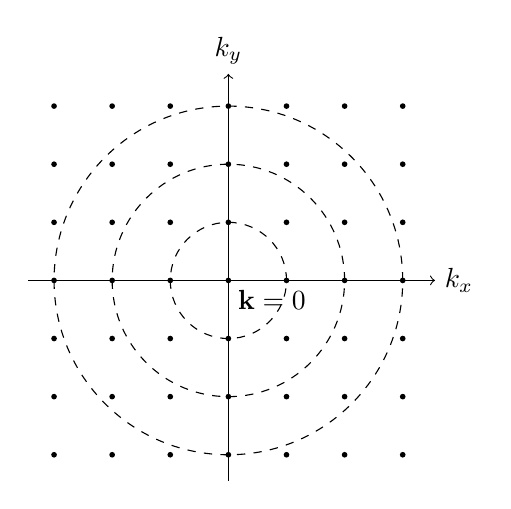
\begin{tikzpicture}[scale=0.82]
\draw[->] (-3.1,0) -- (3.2,0) node[right] {$k_x$};
\draw[->] (0,-3.1) -- (0,3.2) node[above] {$k_y$};
\draw[dashed] (0,0) circle (0.9);
\draw[dashed] (0,0) circle (1.8);
\draw[dashed] (0,0) circle (2.7);
\foreach \x in {-3,-2,-1,0,1,2,3}{
  \foreach \y in {-3,-2,-1,0,1,2,3}{
    \fill (0.9*\x,0.9*\y) circle (1.25pt);
  }
}
\node[below right] at (0,0) {$\mathbf{k}=0$};
\end{tikzpicture}
\caption{Diskrete Impulszustände und Schalen konstanter Energie für Teilchen in einem endlichen periodischen Kasten.}
\end{figure}

Für ein nichtrelativistisches Teilchen gilt
\begin{equation}
E_{\mathbf{k}}=\frac{\mathbf{k}^2}{2m},
\end{equation}
Der Zustand niedrigster Energie ist also \(\mathbf{k}=0\). Setzen wir \(N\) identische Bosonen in den Kasten und suchen den Vielteilchen-Grundzustand. Das erste Boson besetzt den Zustand mit Impuls null. Auch das zweite kann denselben Zustand einnehmen, ebenso das dritte und jedes weitere Boson. Somit besetzen alle \(N\) Bosonen den Zustand \(\mathbf{k}=0\).

Dies ist ein Bosonenkondensat: Eine große Zahl identischer Teilchen besetzt denselben Einteilchenzustand, hier den Zustand niedrigster Energie. Die Wellenfunktion bei verschwindendem Impuls ist räumlich konstant und erstreckt sich über den gesamten Kasten. Sie lokalisiert keines der Bosonen an einem bestimmten Ort; entsprechend ist der Ort jedes Bosons unbestimmt. Bei großer Besetzungszahl baut sich durch die gemeinsame Wellenfunktion eine makroskopische Feldamplitude auf, und das Feld verhält sich zunehmend wie ein klassisches Feld.

Der fermionische Grundzustand sieht völlig anders aus. Betrachten wir zunächst den Fall ohne Spin, sodass jeder Impulsgitterpunkt einem verfügbaren Zustand entspricht. Das erste Fermion besetzt \(\mathbf{k}=0\), doch ein zweites identisches Fermion kann diesen Zustand nicht ebenfalls besetzen. Die nächsten Teilchen müssen Zustände in der nächstniedrigeren Energieschale einnehmen. In einer zweidimensionalen Darstellung gibt es vier nächstgelegene Gitterpunkte mit gleicher Energie, in drei Dimensionen sind es sechs. Sind diese Zustände besetzt, müssen weitere Teilchen in aufeinanderfolgende Schalen eintreten.

Da die Energie proportional zum Quadrat des Abstands vom Ursprung im Impulsraum ist, minimiert man die Gesamtenergie, indem man die besetzten Punkte so nahe wie möglich um \(\mathbf{k}=0\) anordnet, soweit es das Ausschlussprinzip zulässt. Bei vielen Fermionen nähert sich der besetzte Bereich einer Kugel an. Ihre Oberfläche ist die Fermi-Fläche, ihr Inneres das Fermi-Meer und der vollständig besetzte Bereich die Fermi-Kugel. Bei endlichem Volumen ist der Rand etwas unregelmäßig, weil die verfügbaren Punkte ein Gitter bilden. Bei einem großen System wird dieser Effekt jedoch vernachlässigbar.

\begin{figure}
\centering
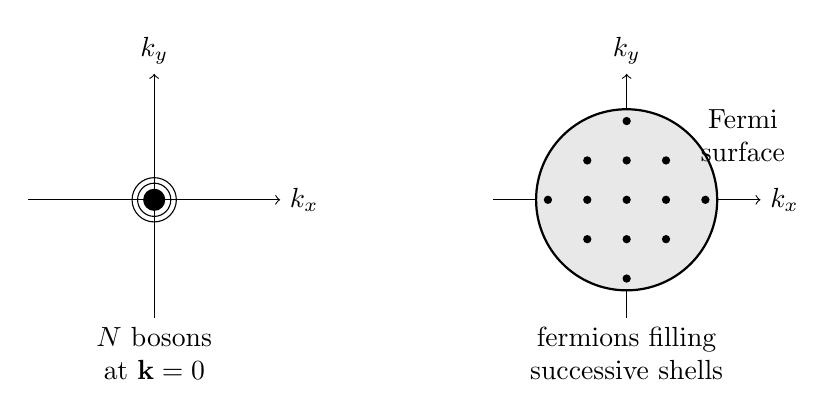
\begin{tikzpicture}[scale=1.0]
\begin{scope}[xshift=-3.0cm]
\draw[->] (-1.6,0) -- (1.6,0) node[right] {$k_x$};
\draw[->] (0,-1.5) -- (0,1.6) node[above] {$k_y$};
\fill (0,0) circle (4pt);
\draw (0,0) circle (6pt);
\draw (0,0) circle (8pt);
\node[align=center] at (0,-1.95) {$N$ bosons\\at $\mathbf{k}=0$};
\end{scope}
\begin{scope}[xshift=3.0cm]
\draw[->] (-1.7,0) -- (1.7,0) node[right] {$k_x$};
\draw[->] (0,-1.5) -- (0,1.6) node[above] {$k_y$};
\fill[gray!18] (0,0) circle (1.15);
\draw[thick] (0,0) circle (1.15);
\fill (0,0) circle (1.5pt);
\fill (0.5,0) circle (1.5pt);
\fill (-0.5,0) circle (1.5pt);
\fill (0,0.5) circle (1.5pt);
\fill (0,-0.5) circle (1.5pt);
\fill (0.5,0.5) circle (1.5pt);
\fill (0.5,-0.5) circle (1.5pt);
\fill (-0.5,0.5) circle (1.5pt);
\fill (-0.5,-0.5) circle (1.5pt);
\fill (1,0) circle (1.5pt);
\fill (-1,0) circle (1.5pt);
\fill (0,1) circle (1.5pt);
\fill (0,-1) circle (1.5pt);
\node[right,align=center] at (0.82,0.82) {Fermi\\surface};
\node[align=center] at (0,-1.95) {fermions filling\\successive shells};
\end{scope}
\end{tikzpicture}
\caption{Bosonen kondensieren im Zustand mit verschwindendem Impuls, während Fermionen die Impulszustände bis zur Fermi-Fläche nach außen auffüllen.}
\end{figure}

Der fermionische Grundzustand hat deutlich mehr Energie als der entsprechende bosonische Grundzustand. Alle Bosonen können bei verschwindendem Impuls bleiben, aber die meisten Fermionen werden in Zustände mit von null verschiedenem Impuls gezwungen. Mit zunehmender Zahl der Fermionen wächst der größte besetzte Impuls. Außerdem enthält eine Schale bei großem Impuls mehr Gitterpunkte als eine Schale nahe dem Ursprung. Eine große Fermi-Kugel umfasst daher viele Teilchen mit beträchtlichem Impuls und nur wenige in den Zuständen mit dem kleinsten Impuls.

Der Unterschied zeigt sich auch bei den angeregten Zuständen. Bei Bosonen erhält man die erste Anregung, indem man ein beliebiges Boson aus dem Kondensat entfernt und in einen angeregten Einteilchenzustand versetzt:
\begin{equation}
(N,0,0,\ldots)\longrightarrow (N-1,1,0,\ldots).
\end{equation}
Es spielt keine Rolle, welches Boson versetzt wird; die Teilchen sind identisch. Höhere Anregungen lassen sich auf verschiedene Arten erzeugen. Je nach Abstand der Energieniveaus kann man ein Boson in ein höheres Niveau oder zwei Bosonen in das erste angeregte Niveau versetzen. Das bosonische System wird angeregt, indem Teilchen aus dem Kondensat in Zustände höherer Energie überführt werden.

Bei Fermionen kann kein Teilchen in einen anderen Punkt innerhalb der gefüllten Fermi-Kugel versetzt werden, denn jeder dieser Punkte ist bereits besetzt. Ein Fermion aus dem Inneren des Fermi-Meeres zu entnehmen und oberhalb der Oberfläche einzusetzen, ist möglich, kostet aber viel Energie. Die energieärmste Anregung entsteht, wenn man ein Fermion knapp innerhalb der Fermi-Fläche entnimmt und in einen unbesetzten Zustand knapp außerhalb versetzt. Das angeregte Elektron hat dann nur wenig Energie oberhalb der Fläche, und der zurückgelassene unbesetzte Zustand liegt nur wenig Energie unterhalb davon.

\begin{figure}
\centering
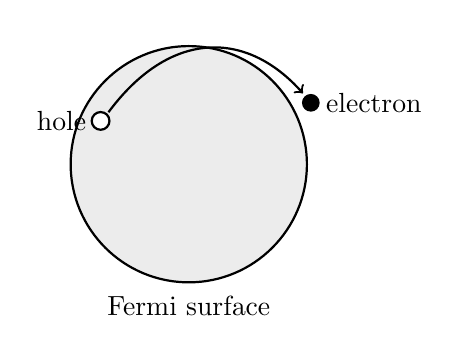
\begin{tikzpicture}[scale=1.0]
\fill[gray!15] (0,0) circle (1.5);
\draw[thick] (0,0) circle (1.5);
\draw[fill=white,thick] (-1.12,0.55) circle (3.2pt);
\fill (1.55,0.78) circle (3.2pt);
\draw[->,thick] (-1.02,0.66) .. controls (-0.25,1.7) and (0.72,1.72) .. (1.45,0.9);
\node[left] at (-1.18,0.55) {hole};
\node[right] at (1.62,0.78) {electron};
\node[below] at (0,-1.55) {Fermi surface};
\end{tikzpicture}
\caption{Bei einer niederenergetischen fermionischen Anregung wird ein Elektron über die Fermi-Fläche gehoben; dabei bleibt ein Loch zurück.}
\end{figure}

\section{Löcher und niederenergetische Anregungen}

Um die Ladung des Lochs anschaulich zu machen, stellen wir uns vor, dass der Kasten gleichmäßig über sein Volumen verteilte positive Ladung enthält. In Materie stammt diese positive Ladung letztlich von den Protonen in den Atomkernen, doch die gleichmäßige Verteilung hält das Modell einfach. Wir fügen so viele Elektronen hinzu, dass sie den Hintergrund neutralisieren. Im Grundzustand füllen diese Elektronen die Fermi-Kugel.

Wenn ein Elektron von unterhalb auf oberhalb der Fermi-Fläche gehoben wird, ändert sich die Gesamtladung des Kastens nicht. Oberhalb der Fläche entsteht ein negativ geladenes Elektron, und unterhalb davon fehlt eine negative Ladung. Das fehlende Elektron lässt sich daher als positiv geladene Anregung behandeln: als Loch.

\begin{classroomqa}
\lecturetimestamp{01:31:38}
\audiencequestion{Hat ein Loch unterhalb der Fermi-Fläche eine negative Energie?}
\lecturerresponse{Nein. Ein Loch ist eine Anregung über dem Vielteilchen-Grundzustand, seine Anregungsenergie ist also positiv. Wird die Energie relativ zur Fermi-Fläche gemessen, kostet es einen positiven Energiebetrag, ein besetztes Elektron unterhalb der Fermi-Fläche zu entfernen.}
\end{classroomqa}

Das entfernte Elektron habe die Energie \(\varepsilon<\varepsilon_F\), das angeregte Elektron die Energie \(\varepsilon'>\varepsilon_F\). Die zugeführte Energie lässt sich in zwei positive Abstände von der Fermi-Fläche zerlegen.\footnote{Die beiden Intervalle werden getrennt angegeben; die hier dargestellte kompakte Gleichung ist eine algebraisch äquivalente Herleitung.}
\begin{equation}
\Delta E
=\varepsilon'-\varepsilon
=(\varepsilon'-\varepsilon_F)+(\varepsilon_F-\varepsilon).
\end{equation}
Der erste Beitrag wird dem Elektron oberhalb der Fermi-Fläche zugeordnet, der zweite dem Loch unterhalb davon:
\begin{equation}
E_{\mathrm{electron}}=\varepsilon'-\varepsilon_F>0,
\qquad
E_{\mathrm{hole}}=\varepsilon_F-\varepsilon>0.
\end{equation}
Das Elektron trägt eine negative, das Loch eine positive Ladung.

Ein Elektron oberhalb der Fermi-Fläche kann später in ein verfügbares Loch fallen. Dabei nimmt seine Energie ab, sodass die frei werdende Energie als Strahlung abgeführt werden muss. Man kann den Vorgang als Übergang eines Elektrons in einen unbesetzten Zustand niedrigerer Energie beschreiben, bei dem ein oder mehrere Photonen emittiert werden. Gleichwertig lässt sich sagen, dass ein Elektron und ein Loch zu Strahlung annihilieren. Das Loch ist kein zusätzlicher fundamentaler Bestandteil des Kastens, sondern eine Abwesenheit im gefüllten Zustand mit vielen Elektronen. Aufgrund seiner Energie und Ladung ist es dennoch nützlich, es als teilchenartige Anregung zu behandeln.

\begin{classroomqa}
\lecturetimestamp{01:36:52}
\audiencequestion{Bedeutet die Anregung eines Elektrons, dass es im Impulsraum von einem Gitterpunkt zu einem anderen versetzt wird?}
\lecturerresponse{Gemeint ist ein Übergang des Elektrons von einem Energieniveau in ein anderes. Bei freien Teilchen im Kasten kennzeichnet das Impulsgitter diese Niveaus, aber die Idee setzt kein Gitter im Impulsraum voraus. In einem Atom ist die positive Ladung im Kern konzentriert. Elektronen besetzen die niedrigsten verfügbaren atomaren Niveaus, und ein Photon kann ein Elektron in ein angeregtes Niveau überführen. Dabei bleibt in dem Niveau, aus dem es kam, ein freier Platz zurück. Dieser freie Platz ist das atomare Gegenstück zu einem Loch.}
\end{classroomqa}

Auch im Kasten wird die Energie eines absorbierten Photons in ein Elektron oberhalb der Fermi-Fläche und ein Loch unterhalb davon umgewandelt. Im Atom beschreibt dieselbe Ausdrucksweise das angeregte Elektron zusammen mit dem freien Platz, der in den zuvor besetzten niedrigeren Niveaus zurückbleibt.

\begin{classroomqa}
\lecturetimestamp{01:39:16}
\audiencequestion{Kann ein niederenergetisches Photon von einem Elektron irgendwo in der Fermi-Kugel absorbiert werden?}
\lecturerresponse{Nein. Liegt das Elektron tief im Fermi-Meer, sind alle benachbarten Zustände bereits besetzt, und ein niederenergetisches Photon kann es nicht bis zu einem unbesetzten Zustand oberhalb der Oberfläche anheben. Nur Elektronen nahe genug an der Fermi-Fläche haben zugängliche leere Zustände innerhalb des Energiebereichs des Photons. Ein ausreichend energiereiches Photon kann ein Elektron aus dem Inneren des Fermi-Meeres anregen.}
\end{classroomqa}

Der Absorptionsquerschnitt bei niedrigen Energien wird daher von der Oberfläche des Fermi-Meeres bestimmt und nicht von seinem gesamten Volumen. Elektronen tief im Fermi-Meer können keine kleinen Übergänge vollziehen; Elektronen knapp unterhalb der Oberfläche lassen sich knapp über sie heben.

\begin{classroomqa}
\lecturetimestamp{01:40:42}
\audiencequestion{Was hindert Elektronen daran, ohne ein einfallendes Photon direkt miteinander zu wechselwirken?}
\lecturerresponse{Nichts. Elektron--Elektron-Wechselwirkungen werden in diesem einfachen Modell vernachlässigt, weil das Fermi-Meer-Bild dadurch komplizierter würde. In dieser ersten Näherung für ein Metall wird ihr effektiver Einfluss als so schwach behandelt, dass er meist ignoriert werden kann.}
\end{classroomqa}

\begin{classroomqa}
\lecturetimestamp{01:41:10}
\audiencequestion{Was geschieht, wenn ein Photon genügend Energie besitzt, um mehrere Elektronen anzuregen?}
\lecturerresponse{Grundsätzlich ist jeder mit den Erhaltungssätzen vereinbare Prozess möglich. Das Photon kann mehr als ein Elektron--Loch-Paar erzeugen: Werden zwei Elektronen angeregt, bleiben auch zwei Löcher zurück. Bei einem solchen Prozess entstehen mehr Anregungen; er ist im Allgemeinen weniger wahrscheinlich, als die Energie zur deutlich stärkeren Anregung eines einzelnen Elektrons zu verwenden.}
\end{classroomqa}

\begin{classroomqa}
\lecturetimestamp{01:42:06}
\audiencequestion{Können zwei Photonen gemeinsam absorbiert werden, wenn keines von beiden allein die Anregung bewirken kann?}
\lecturerresponse{Ja. Absorption ist probabilistisch, und ein Zwei-Photonen-Prozess kann auftreten, wenn die kombinierte Photonenenergie eine verfügbare Anregung erreicht, obwohl jedes Photon für sich unter der erforderlichen Energie bleibt. Reicht die Energie des verfügbaren Lichts nicht aus, um irgendeine erlaubte Anregung zu erreichen, durchdringt es das System weitgehend.}
\end{classroomqa}

\editorialnote{Eine kurze Erörterung an dieser Stelle stellt einen Zusammenhang zwischen absorbierter Strahlung und der kollektiven Bewegung von Elektronen her; die inhaltlichen Einzelheiten lassen sich jedoch nicht wiedergewinnen. Gesichert ist lediglich die Aussage, dass eine solche kollektive Antwort komplizierter ist als das Einzelteilchen--Loch-Bild.}

\begin{classroomqa}
\lecturetimestamp{01:43:49}
\audiencequestion{Warum gelten Elektron--Elektron-Wechselwirkungen als schwach, wenn alle Elektronen dieselbe negative Ladung tragen?}
\lecturerresponse{Die Elektronen befinden sich in einem kompensierenden positiven Hintergrund. Dieser schirmt die Ladung eines Elektrons ab und verringert in dieser vereinfachten Situation die effektive Wechselwirkung. Die Wechselwirkung verschwindet nicht; für ihre Behandlung muss die Abschirmantwort des Mediums berücksichtigt werden.}
\end{classroomqa}

\begin{classroomqa}
\lecturetimestamp{01:44:41}
\audiencequestion{Wird die Abschirmung später behandelt?}
\lecturerresponse{Ja. Die Abschirmung ist wichtig, wird aber zurückgestellt, bis sich das wechselwirkende System umfassender behandeln lässt.}
\end{classroomqa}

\section{Ein fermionisches Meer in einer Dimension und Antiteilchen}

Die Konstruktion mit Löchern führt zu Antiteilchen. Dieselbe logische Struktur lässt sich von Elektronen in Materie auf ein relativistisches Quantenfeld und sein Vakuum übertragen. Die einfachste Version betrachtet ein masseloses fermionisches Feld \(\psi(x,t)\) in einer Raumdimension. In Einheiten, in denen die Lichtgeschwindigkeit eins ist, lauten die beiden möglichen linearen Dispersionsrelationen
\begin{equation}
\omega=k,
\qquad\text{or}\qquad
\omega=-k.
\end{equation}
Zunächst betrachten wir ausdrücklich den ersten Zweig.

\editorialnote{Im abschließenden Austausch wechseln sich miteinander unvereinbare Identifikationen der Teilchen ab. Als gesichert gilt ein nicht näher spezifiziertes masseloses fermionisches Modellfeld in einer Raumdimension, beschränkt auf eine Ausbreitungsrichtung.}

Für eine ebene Welle
\begin{equation}
\psi(x,t)=e^{i(kx-\omega t)},
\end{equation}
lauten die Ableitungen
\begin{equation}
\frac{\partial\psi}{\partial t}=-i\omega\psi,
\qquad
\frac{\partial\psi}{\partial x}=ik\psi.
\end{equation}
Damit ist \(\omega=k\) äquivalent zur Differentialgleichung erster Ordnung für das Feld
\begin{equation}
\frac{\partial\psi}{\partial t}
=-\frac{\partial\psi}{\partial x}.
\end{equation}

\begin{figure}
\centering
\includegraphics[width=0.72\textwidth]{lecture_05_figure_05.png}
\caption{Beginn der Differentialgleichung erster Ordnung für das Feld, deren ebene Wellen \(\omega=k\) erfüllen.}
\lectureframe{01:47:22}
\end{figure}

Jedes Profil der Form \(f(x-t)\) erfüllt diese Gleichung und breitet sich nach rechts aus. Bei umgekehrtem Vorzeichen gilt
\begin{equation}
\frac{\partial\psi}{\partial t}
=+\frac{\partial\psi}{\partial x},
\end{equation}
Die Profile \(f(x+t)\) breiten sich nach links aus. Jede der beiden Differentialgleichungen erster Ordnung wählt nur eine Ausbreitungsrichtung aus. Nehmen wir an, das Feld sei fermionisch und seine Teilchen trügen, für das Argument mit den Löchern, elektrische Ladung.

Der Zweig \(\omega=k\) führt unmittelbar zu einem Problem. Die Wellenzahl \(k\) kann negativ sein, und daher kann auch \(\omega\) negativ sein. Da \(\omega\) in diesen Einheiten die Energie ist, enthält das geradlinige Spektrum sowohl Zustände positiver als auch negativer Energie:
\begin{equation}
E=\omega=k.
\end{equation}

\begin{figure}
\centering
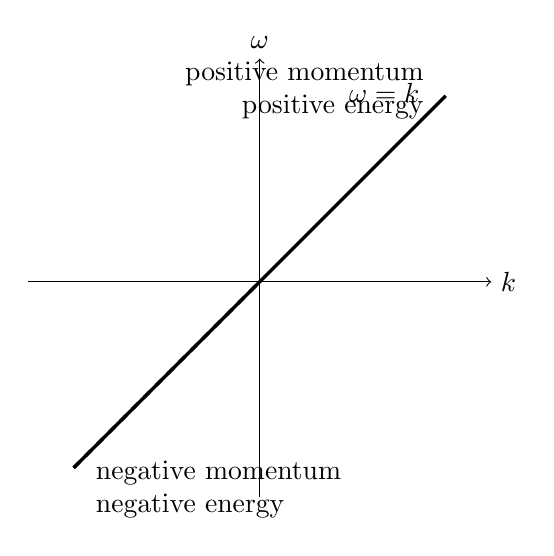
\begin{tikzpicture}[scale=1.05]
\draw[->] (-2.8,0) -- (2.8,0) node[right] {$k$};
\draw[->] (0,-2.6) -- (0,2.7) node[above] {$\omega$};
\draw[very thick] (-2.25,-2.25) -- (2.25,2.25);
\draw[very thick,dashed] (-2.25,-2.25) -- (0,0);
\node[above left] at (2.05,2.05) {$\omega=k$};
\node[below right,align=left] at (-2.1,-2.05) {negative momentum\\negative energy};
\node[above left,align=right] at (2.1,1.85) {positive momentum\\positive energy};
\end{tikzpicture}
\caption{Das Spektrum des einzelnen Zweigs \(\omega=k\) mit seiner Hälfte negativer Energien bei \(k<0\).}
\end{figure}

Ein gewöhnliches leeres Vakuum kann nicht der Grundzustand einer solchen Theorie sein. Ein Fermion positiver Energie könnte ein Photon abstrahlen und in einen niedrigeren Zustand übergehen. Nichts würde es bei null aufhalten: Es könnte weiter in Zustände negativer Energie übergehen, noch mehr Strahlung emittieren und unbegrenzt weiter abfallen. Die vom Fermion abgegebene Energie erschiene im Strahlungsfeld. Ein nach unten unbeschränktes Spektrum bietet daher kein stabiles gewöhnliches Vakuum.

Das Ausschlussprinzip für Fermionen ermöglicht einen anderen Ausgangspunkt. Besetzen wir jeden Einteilchenzustand negativer Energie bis hinauf zu null mit einem Fermion. Kein weiteres Fermion kann in diese Zustände fallen, da jeder bereits besetzt ist. Ein weiteres Fermion negativer Energie hinzuzufügen ist unmöglich, während das Hinzufügen eines Fermions positiver Energie die Energie erhöht. Das vollständig gefüllte Meer negativer Energien kann daher als Vielteilchen-Grundzustand betrachtet und Vakuum genannt werden.

\begin{figure}
\centering
\resizebox{\linewidth}{!}{%
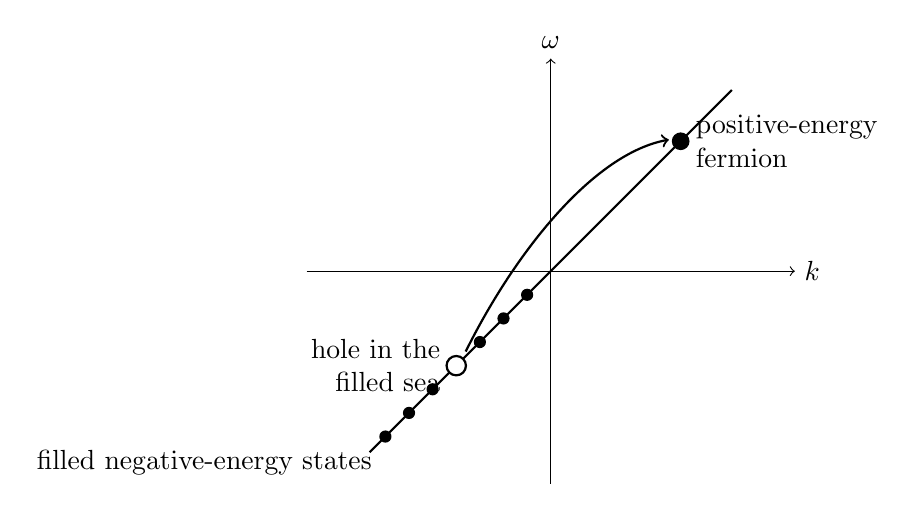
\begin{tikzpicture}[scale=1.0]
\draw[->] (-3.1,0) -- (3.1,0) node[right] {$k$};
\draw[->] (0,-2.7) -- (0,2.7) node[above] {$\omega$};
\draw[thick] (-2.3,-2.3) -- (2.3,2.3);
\foreach \p in {-2.1,-1.8,-1.5,-1.2,-0.9,-0.6,-0.3}{
  \fill (\p,\p) circle (2.2pt);
}
\draw[fill=white,thick] (-1.2,-1.2) circle (3.5pt);
\fill (1.65,1.65) circle (3.2pt);
\draw[->,thick] (-1.08,-1.02) .. controls (-0.45,0.25) and (0.55,1.5) .. (1.5,1.67);
\node[left,align=right] at (-1.28,-1.2) {hole in the\\filled sea};
\node[right,align=left] at (1.72,1.65) {positive-energy\\fermion};
\node[below left] at (-2.15,-2.15) {filled negative-energy states};
\end{tikzpicture}%
}
\caption{Das gefüllte Meer negativer Energien und eine Anregung, bei der ein Fermion in einen Zustand positiver Energie gehoben wird.}
\end{figure}

Die einfachste Anregung entsteht, indem man ein Fermion aus dem Meer negativer Energien entfernt und in einen Zustand positiver Energie versetzt. Das angeregte Fermion ist ein gewöhnliches Teilchen positiver Energie. Die zurückbleibende Leerstelle im Meer ist eine zweite Anregung: ein Loch. Ist das entfernte Fermion negativ geladen, so ist das Loch positiv geladen.

In diesem Beispiel mit einem einzigen Zweig hat das Loch auch positiven Impuls. Besetzte das fehlende Fermion einen Zustand mit Impuls \(k_-<0\), ändert sich der Gesamtimpuls durch seine Entfernung um
\begin{equation}
p_{\mathrm{hole}}=-k_->0.
\end{equation}
Es handelt sich also um ein Defizit an negativem Impuls. Die Anregung besteht somit aus einem Fermion mit positiver Energie und negativer Ladung sowie einem Loch mit positiver Energie und positiver Ladung. Beide tragen positiven Impuls und bewegen sich auf dem Zweig \(\omega=k\) nach rechts.

In der vollständigen Elektronentheorie ist das positiv geladene Loch das Positron. Dirac zog zunächst in Betracht, das Loch mit dem Proton zu identifizieren. Die Konstruktion verlangt, dass ein Teilchen und sein Antiteilchen dieselbe Masse haben. Das Loch ist ein eigenständiges Teilchen mit der Masse des Elektrons und entgegengesetzter elektrischer Ladung. Dies ist die grundlegende Teilchen--Antiteilchen-Deutung, zu der das Spektrum negativer Energien führte.

Dieselbe Rettung lässt sich nicht auf Bosonen übertragen. Ein bosonischer Zustand kann beliebig viele Teilchen enthalten; deshalb gibt es keine Möglichkeit, ein Niveau negativer Energie einmalig zu füllen und so eine weitere Besetzung zu verhindern. Es könnten stets weitere Bosonen zu diesem Niveau hinzugefügt werden, wodurch die Energie immer weiter sänke:
\begin{equation}
\begin{aligned}
\text{fermionic mode: }&n=0\ \text{or}\ 1,\\
\text{bosonic mode: }&n=0,1,2,\ldots .
\end{aligned}
\end{equation}
Das vorgeschlagene bosonische System hätte weiterhin keinen Grundzustand. In dieser elementaren Konstruktion beruht die Stabilität des gefüllten Meeres genau auf dem Ausschlussprinzip für Fermionen.

Diese Gleichung in einer Dimension ist nur eine Modellversion der Dirac-Gleichung. Ihr Feld ist masselos, bewegt sich mit Lichtgeschwindigkeit und breitet sich nur in einer Richtung aus. Eine vollständigere Dirac-Gleichung muss die fehlenden Bewegungsrichtungen und die übrige relativistische Teilchenstruktur berücksichtigen. Auf diese umfassendere Gleichung und die Behandlung von Antiteilchen bosonischer Felder wird später eingegangen.
